\documentclass[11pt,a4paper]{article}
\usepackage{ls}
\usepackage[english]{babel}
\setlist{noitemsep}

\title{Business Model Patterns and Sustainability}  

\author{Hans-Gert Gr\"abe}
\date{06 May 2022}

\begin{document}
\maketitle
\tableofcontents
\newpage

\section{Basics on Institutionalisation Processes}

\subsection{Dynamics of the Levels of Our Technology Definition}

Technology was defined in the lecture as interrelation of
\begin{itemize}
\item globally available \emph{procedural knowledge}, 
\item \emph{institutionalised procedures} ("state of the art") and
\item private \emph{procedural skills}.
\end{itemize}

The dynamics of these levels are closely linked:
\begin{enumerate}
\item Private procedural skills are based on institutionalised practices from
  which \emph{justified expectations} are derived.
\item The use of private procedural skills leads to \emph{experienced
  results}. Comparing them with justified expectations influences the
  institutionalisation of practically successful actions as proven practices.
\item This empiricism is \emph{condensed and generalised} as procedural
  knowledge extending it with appropriate conceptual systems, which in turn
  has an influence on the further development of "reasonable" practices and
  their forms of institutionalisation as \emph{contexts of justification}.
\end{enumerate}

\subsection{Transformation of Practically Proven into Proven Practices}

The transformation of what is practically proven into proven practices follows
a general line:
\begin{enumerate}
\item Procedures are standardised as processes and enhanced with appropriate
  conceptual systems and thus become comparable.
\item Tools are developed to support the operation of these processes.
\item Problems in the operation of these procedures are analysed, solutions
  are generalised, the practically proven is condensed into \emph{patterns}
  and further into standards, norms and the \emph{state of the art}.
\end{enumerate}
The generalisation of isolated practices into patterns also plays a role in
the TRIZ process model (Fig. 1): Darrell Mann's \emph{Select} phase draws on
these generalised experiences, which, however, for the TRIZ \emph{user} only
play a role as proven practices. Scientific elaboration means both empirically
to consolidate these proven practices and to integrate them into broader
contexts of justification and to develop corresponding conceptual worlds.

\subsection{Patterns and Contexts}

These forms of institutionalisation are embedded as initially domain-specific
patterns in a \emph{domain-specific} methodology, for example as industry
sector-specific standards and thus are \emph{contextualised}.  These patterns
can be further generalised to cross-domain standards such as the APQC PCF as a
Cross-Industry Process Classification Framework \cite{APQC}.  However, this is
also \emph{not universally valid}, but contextualised itself, as it still
refers to organisations of a specific-general design.

\begin{center}
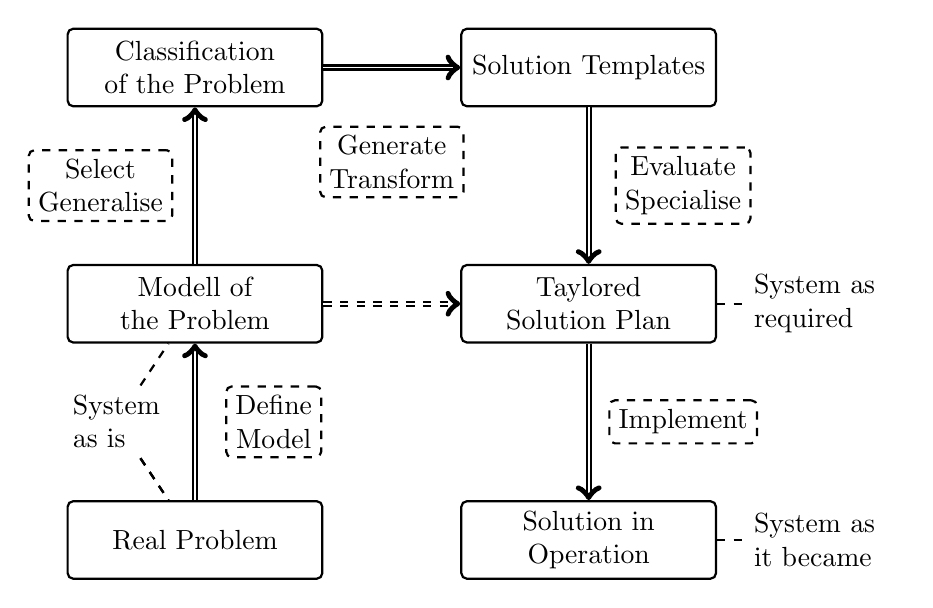
\begin{tikzpicture}[%scale=.95,transform shape,
    textbox/.style={draw, text width=3cm, minimum height=2.8em,
      align=center},
    ovalbox/.style={draw, dashed, align=center},
    %>={Triangle[length=0pt 6,width=0pt 5]},
    rounded corners=2pt,line width=.8pt]

  \node[text width=1.1cm] at (-1,1.5) (A0) {System\\ as is};
  \node[textbox] at (0,0) (A1) {Real Problem};
  \node[ovalbox] at (1,1.5) {Define\\ Model}; 
  \node[textbox] at (0,3) (A2) {Modell of the Problem};
  \node[ovalbox] at (-1.2,4.5) {Select\\ Generalise}; 
  \node[textbox] at (0,6) (A3) {Classification of the Problem};
  \node[ovalbox] at (2.5,4.8) {Generate\\ Transform}; 
  \node[textbox] at (5,6) (B3) {Solution Templates};
  \node[ovalbox] at (6.2,4.5) {Evaluate\\ Specialise}; 
  \node[textbox] at (5,3) (B2) {Taylored\\ Solution Plan};
  \node[ovalbox] at (6.2,1.5) {Implement}; 
  \node[textbox] at (5,0) (B1) {Solution in Operation};
  \node[text width=1.8cm] at (8,3) (C2) {System as\\ required};
  \node[text width=1.8cm] at (8,0) (C1) {System as\\ it became};

  \draw[-,dashed] (A0) -- (A1);
  \draw[-,dashed] (A0) -- (A2);
  \draw[-,dashed] (B1) -- (C1);
  \draw[-,dashed] (B2) -- (C2);
  \draw[-,dashed] (A0) -- (A1);
  \draw[-,dashed] (A0) -- (A1);

  \draw[double,->] (A1) -- (A2) ;
  \draw[double,->] (A2) -- (A3) ;
  \draw[double,->] (A3) -- (B3) ;
  \draw[double,->,dashed] (A2) -- (B2) ;
  \draw[double,->] (B3) -- (B2) ;
  \draw[double,->] (B2) -- (B1) ;
\end{tikzpicture}\\[1em]
Fig. 1: The TRIZ Process Model
\end{center}

\subsection{TRIZ and Patterns}

TRIZ is similarly structured. It comes with a toolbox of problem-solving
patterns (Select in \cite{Mann})
\begin{itemize}
\item Inventive principles
\item Separation Principles
\item Inventive standards for SF models
\item Evolution patterns of technical systems
\item Evolution trends
\item Functional-analysis based trimming,
\end{itemize}
but assumes a specific type of modelling (Define in \cite{Mann}) with
\begin{itemize}
\item Systemic delimitation
\item Ideality
\item Focussing of an operative zone
\item Action and evaluation parameters in functional modelling
\item Description of problems as contradictory behaviour of evaluation
  parameters when action parameters change.
\end{itemize}
Only on the basis of this (Define) the (Select) is possible. It is also not
only a matter of \emph{selecting} the patterns suitable for the solution, but
also of \emph{selecting proven applicable methodological procedures} that are
based on the respective patterns.
\newpage

\section{Development of Business Process Modelling}

When we talk about Business TRIZ today, we are talking about a similar
development of institutionalisation of structuring procedures in the area of
business processes.  In the context of P-TRIZ (Seminar on 9 May 2022), we had
identified three stages of that development.

\paragraph{1.}
With the transition to more advanced forms of industrial production at the
beginning of the 20th century, individual work processes were deconstructed,
charged with forms of description and assembled into new "living" systems --
the \emph{assembly line system} of modern industrial production. The control
of the complex interrelationships in such an organisation remained as "art of
management" beyond the realm covered by these structural standardisation of
work processes.

Together with this institutionalisation complex engineering disciplines such
as process engineering or automation technology emerged, which are concerned
not only with the processes themselves, but also are developing the tools
(understood in a comprehensive sense) that have been and are being used in the
context of this institutionalisation.

With its procedures and patterns, classical TRIZ aims at problem solving in
this area. It can be applied only if the concrete application domain is
conceptually penetrated to such an extent that the specific type of modelling
required in the TRIZ analysis phase can be carried out.  In this sense TRIZ is
a "scientific method".

"Management" remains an art, as for example in "Mintzberg on Management"
\cite{Mintzberg}. Certainly an artist must master the \emph{technical
  procedures} of his subject, but the practical combination of such techniques
remains at the level of private procedural skills.

\paragraph{2.}
Since the 1960s, the structuring of procedures in the operational management
of individual companies has gained in importance as \emph{business process
  modelling}.

These institutionalisation processes are not possible without the preceding
institutionalisations of the technical core processes and build on them.

Howard Smith \cite{Smith2006} stated in 2006 that these institutionalisation
processes are well advanced with the development and widespread use of
computer-based Business Process Management (BPM) systems and the establishment
of uniform conceptual systems such as the APQC PCF \cite{APQC}. According to
Howard Smith this allows to move on to the next level, to \emph{P-TRIZ}.
\begin{quote}
  P-TRIZ is the application of modern TRIZ towards business process
  improvement, innovation, and transformation. Coupled to BPM methods, it
  provides the engineering discipline that amplifies the creativity of those
  who seek to re-design processes. \cite{Smith2006}
\end{quote}
  
\paragraph{3.}
In the management literature, this level of institutionalisation of
structuring in inter-company cooperation has since been roughly associated
with the term \emph{Business Model}. It is based on the forms of
institutionalisation of intra-company operative business, but did not develop
as quickly as Howard Smith expected in \cite{Smith2006}.

\section{Business Process Models and Business Models}

\subsection{Business Process Models}

The confusion between these two levels of generalisation is also reflected in
the literature consulted for the seminar.  In \cite{Fellmann2018}, "business
process model patterns" are examined, which are defined as
\begin{quote}
  the description of a proven solution to a recurring problem that is related
  to the creation or modification of business process models in a specific
  context. This description is typically organised in a structured document
  supporting the reader in understanding under which circumstances the
  proposed solution will be useful (ibid, p. 974),
\end{quote}
The authors clearly emphasise that 
\begin{quote}
  in economics the term \emph{business model patterns} is used for a pattern
  describing the economic principles of an organisation [\ldots] Although
  business model patterns can be depicted visually, they were not considered
  in our survey due to their specificity on the economics perspective.
\end{quote}
The aim of \cite{Fellmann2018} is described as to "discuss patterns related to
various aspects of process modeling" (ibib, p. 981). Hence even 15 years after
\cite{Smith2006}, the third phase of the institutionalisation of patterns is
still a prominent topic as a central component of problem-solving in the field
of Business Process Landscapes of operational management.

\emph{Patterns} are understood in the sense of Christopher Alexander's
architecture patterns \cite{Alexander} or the Software design patterns of the
"Gang of Four" \cite{Gamma}:  
\begin{quote}
  A pattern is a combination of a problem and a corresponding solution that is
  described in a systematic and generic way, so that it can be used over and
  over again in different situations. \cite[p. 3]{LF2018}
\end{quote}

This is not exactly the same as principles, evolutionary lines or trends in
TRIZ, as in these approaches there is no direct link between problem and
solution, but the "TRIZ model of the system as it is" is used as starting
point for selecting a systemic transformation pattern first to design the
solution in general and then to concretise it with available resources (phase
\emph{Select} in \cite{Mann} -- see the descriptions of the different
\emph{Problem Solving Tools} there).  These tools are nevertheless also
subsumed as "patterns" below.

Business TRIZ has a similar focus as business process models in many practical
applications in which it has to resolve contradictory objectives in the
operational organisation of the company. However, Business TRIZ does not look
for new patterns, but tries to transfer the patterns known from the technical
field to this field and adapt them on the basis of new domain-specific
experience. Such a transfer may seem suspicious at first glance.  However, it
can be observed that essential instruments of classical TRIZ, such as, e.g.,
the Patterns of Evolution of Technical Systems, are based on observations on
market processes and developments as explained in more detail in
\cite{Graebe2020} and thus have a certain relevance not only for the level of
Business Process Management Systems but also for the level of Business Models.

\subsection{Business Models}

The level of business models has been studied more intensively since around
2010. In a first overview \cite{Zott2011} the authors observed "that scholars
do not agree on what a business model is, and that the literature is
developing largely in silos, according to the phenomena of interest to the
respective researchers". They present a list of eight different definitions of
the notion of a business model and identified emerging common themes among
scholars of that area:
\begin{enumerate}
\item The notion of business model is emerging as a new unit of analysis.
\item Business models emphasise a system-level, holistic approach towards
  explaining how firms “do business”.
\item Firm \emph{activities} play an important role in the various
  conceptualisations of business models that have been proposed.
\item Business models seek to explain how value is created, not just how it is
  captured. 
\end{enumerate}

This strong orientation of business model (patterns) towards value creation
plays a central role in \cite{Remane2019}, \cite{Zott2011}, but also in the
much-cited reference \cite{Gassmann2014}. Despite such a relatively
homogeneous focus, however, no generally accepted "Pattern Database" has yet
emerged.  One problem is, of course, the focus itself, since \emph{value
  proposition} is oriented towards a functional property of the components and
not towards a functional property of the network, whose \emph{main useful
  function} should be an emergent function of the network as a whole according
to the theoretical approach of TRIZ.

\section{Business Models and Sustainability}

In this sense, the concept of sustainability is a touchstone to what extent
Business Model Pattern taxonomies can address topics beyond such a narrow
focus.

Today's inclusion of sustainability issues in business models is largely the
result of a longer-term politicisation of this issue.

\subsection{Sustainability Emerging as Business Goal}

The importance of sustainable and ecological aspects in management has been a
topic of public awareness at least since the reports on the \emph{Limits to
  Growth} by the Club of Rome. While in the early years the debate focused on
the finiteness of available natural resources and thus on longer-term
development aspects of availability of a \emph{material basis} (such as "Peak
Oil"), in the last 20 years it has become increasingly visible that global
\emph{processes} (such as "climate change" or "extinction of species") will
leave established ranges much earlier if the currently active industrial mode
of production which is the basis of our prosperity will be followed up without
substantial changes.  

In contrast to other globalisation processes such as, e.g., the implementation
of Intellectual Property Rights, these processes do not originate and were not
driven by individual interest groups, but have the \emph{cooperative action}
of an inherently global "thinking community" of a networked, interdisciplinary
science as their basis. The problematisation was initiated and formed by
transnational political bodies and today plays an increasingly important role
in the framework of international political affairs. The formula "think
globally, act locally" nevertheless expresses that those global challenges can
only be met through changed local action. Corresponding awareness-raising
processes at the socio-cultural and political level have meanwhile reached
such a degree that at least a financially potent middle class bases its
economic decisions also on ecological and social issues.

With the 17 Sustainable Development Goals (SDG) adopted in 2015 by the UN, the
politicisation of this issue has reached a new dimension, as these goals
anchor long-term objectives of necessary changes with today's cooperative
actions.

\begin{center}
  \begin{minipage}{.55\textwidth}\centering
    \includegraphics[width=\textwidth]{images/SDG.png}\\
    Sustainable Development Goals
  \end{minipage}\hfill
  \begin{minipage}{.4\textwidth}\centering
    \includegraphics[width=\textwidth]{images/Triple-Bottom-Line.png}\\[1em]
    Triple Bottom Line
  \end{minipage}
\end{center}

\subsection{Sustainability and Business Models}

In the business environment and more general socio-economic debates, this
politicisation is anchored with the slogan of the \emph{Triple Bottom Line:
  Planet -- People -- Profit} \cite{Elkington1997}. It obviously reveals
massive contradictory dimensions in the inclusion of ecological (planet) and
social (people) goals into economic processes.

Even if such a narrative is being further refined today with the PESTLE
approach (addressing the political, economical, social, technological, legal
and environmental dimensions), in view of the value orientation of Business
Model Pattern taxonomies so far, a consistent orientation towards all three
"P" can hardly be expected.

This main focus on value propositions is emphasised in \cite{LF2018} in the
introduction to the survey citing \cite{Schaltegger2016}:
\begin{quote}
  A business model for sustainability “helps describing, analyzing, managing,
  and communicating
  \begin{itemize}
  \item[(i)] a company’s sustainable value proposition to its customers, and
    all other stakeholders,
  \item[(ii)] how it creates and delivers this value,
  \item[(iii)] and how it captures economic value while maintaining or
    regenerating natural, social, and economic capital beyond its
    organizational boundaries”.
  \end{itemize}
\end{quote}
The authors extraced 45 patterns from the literature on Sustainable Business
Models and grouped them into 11 pattern groups
\begin{itemize}
\item[G1] Pricing \& Revenue Patterns (4 patterns)
\item[G2] Financing Patterns (3 patterns)
\item[G3] Ecodesign Patterns  (4 patterns)
\item[G4] Closing-the-Loop Patterns (9 patterns)
\item[G5] Supply Chain Patterns (6 patterns)
\item[G6] Giving Patterns (2 patterns)
\item[G7] Access Provision Patterns (6 patterns)
\item[G8] Social Mission Patterns (5 patterns)
\item[G9] Service \& Performance Patterns (4 patterns)
\item[G10] Cooperative Patterns (1 pattern)
\item[G11] Community Platform Patterns (1 pattern)
\end{itemize}
As example the patterns in the group \emph{Pricing \& Revenue Patterns} are
listed: 
\begin{itemize}
\item Differential Pricing
\item Freemium
\item Innovative Product Financing
\item Subscription Model
\end{itemize}
According to the pattern definition for each of the patterns context, problem
and solution are described and an example is given, e.g. for
\emph{Differential Pricing}
\begin{itemize}
\item \emph{Context:} Base of the Pyramid and low-income groups in both
  developed and developing countries are often excluded from consumption due
  to price barriers.
\item \emph{Problem:} Customers might need the same product but have different
  payment thresholds. Hence, some customers are either unwilling or unable to
  pay as much as others for the same product.
\item \emph{Solution:} Charging groups with higher payment thresholds higher
  prices to subsidize those groups who cannot afford to pay as much.
\item \emph{Example:} [Novo Nordisk] sells insulin in developing countries at
  prices that are up to 20\% below the mean prices charged in developed
  countries.
\end{itemize}

The example shows very well the structured approach (the patterns are
available in RDF notation in the WUMM database), but also the extensive
orientation towards new and flexible forms of value proposition, which are
driven more by new possibilities which emerge within digital change than by
questions of sustainability.  This is also emphasised in
\cite[p. 3]{Russo2020}:
\begin{quote}
  General purpose idea generation tools do not usually show any specific
  preference to sustainable aspects, since their overall purpose is product
  success and the identification of unexplored market opportunities.
  Therefore, the attention to sustainability is random, not taken for granted
  and presumably dependent on designers’ sensibilities towards environmental
  and human problems.
\end{quote}

\section{Eco Design Principles}

\subsection{Lifecycle Orientation and Eco Design Principles}

The approach in \cite{Russo2020} is very different.  Over several years the
authors worked out and consolidated \emph{Eco Design Principles} (EDP).  The
focus is not on Business Models but on the Product Lifecycle and thus on
\emph{material processes} in their full complexity. Even if "market success as
key for any eco-design product" \cite[p. 1]{Maccioni2019} is emphasised, the
EDP are primarily directed at the early phases of product design.  Hence it is
difficult to assess the impact on "value proposition" and market success.  See
\cite{Maccioni2019} for an evaluation of such aspects.

The general orientation of EDP is described in \cite[p. 3]{Russo2020} as
follows:
\begin{quote}
  During design phase, each designer is supposed to follow a list of
  guidelines and accordingly modify the existing product to make it more
  environmentally friendly. The crucial point is to exploit problem solving
  strategies as a framework for eco-guidelines that guide the user to make
  product development, taking into account first of all sustainability
  objectives.

  It is important to understand that problem-solving tools are not easy to
  learn, so a strong simplification is needed to guide non-experts. Unlike a
  structured problem-solving method that involves a preliminary phase of
  understanding and modeling the problem, an eco-guideline acts exclusively as
  an inventive trigger. Therefore, it must be both simple to understand and
  effective.
\end{quote}

The aim of the EDP presented in \cite{Russo2020} is "the customization of a
set of tools that are typical of the TRIZ methodology. Almost all suggestions
are based on TRIZ tools [\ldots] However, TRIZ is not a method born to do
Ecodesign and, therefore, there has been a long work of selection and
adaptation of individual instruments. Only those instruments leading to
solutions with less waste of resources have been chosen."

16 generic strategies are derived,
\begin{enumerate}
\item Switch to super system
\item Trimming
\item Dematerialization/ideality
\item Merging
\item Redesign the internal structure
\item Change the state of aggregation
\item Local quality
\item Substitute
\item Segmentation of the parts/components
\item Design for Assembly
\item Dynamics
\item The Other Way Around
\item Taking out
\item Increase control
\item Recycle/Reuse
\item Optimize
\end{enumerate}
to which the identified 59 Eco Guidelines are assigned. Each of these generic
strategies is embedded in the TRIZ methodology and their solving power is
outlined without, however, assigning them to a problem.

Example: Strategy 2 \emph{Trimming}:
\begin{quote}
  Trimming is a good technique for making greener products. It consists of
  making a product constituted by fewer parts, with positive consequences on
  many aspects of the product life cycle, from the management of warehouse
  orders, storage, transport, as well as on reducing the mass. In order to
  achieve the maximum environmental benefits, it is preferable to start by
  eliminating those pieces having the highest impact on the environment. When
  a component is deleted from the system, it is better to try to exploit the
  resources already available in the super-system to replace its useful
  function.
\end{quote}

The authors emphasise that they "have worked on the mechanisms of activation
of creativity that are typical of the TRIZ methodology, trying to translate it
into guidelines bypassing every step of problem definition." This is clearly
different to the "pattern approach" as developed, e.g., in \cite{LF2018}.

The description of each principle contains a detailed \emph{Generic
  Suggestion}, more structured \emph{specific suggestions} and examples.

Similar to \cite{Gassmann2014}, the individual EDPs are also assigned values
from a morphological table with the attributes \emph{when, action, what,
  how}.
\begin{itemize}
\item \emph{When:} Premanufacturing, Manufacturing, Use, End of Life
\item \emph{Action:} Eliminate, Reduce Mass, Reduce Volume, Reduce Quantity,
  Reduce Distance, Improve Durability, Select Other.
\item \emph{What:} Raw materials, External logistics, Internal logistics,
  Packaging, Machineries, Auxiliary materials, Components, Emissions, Energy.
\item \emph{How:} Generic suggestion, Resources list, Example.
\end{itemize}
The general pattern of a guideline is formulated as 
\begin{quote}
  (WHEN) you want to intervene, (ACT) on components (WHAT), by doing
  something (HOW) and using one resource (from the Resource list) to find
  alternatives and assess environmental impacts.  
\end{quote}
In \cite[Fig. 2]{Russo2020} the following sample of a guideline is given: 
\begin{quote}
  During supply task (WHEN -- Premanufacturing),\\ reduce the mass (ACTION --
  Reduce mass)\\ of the raw material (WHAT -- Raw material)\\ by recycling
  waste material in your facility to make it new raw material for the product
  (HOW -- Generic Suggestion). \\
  See list of structural resources (HOW -- Resources list)\\
  In order to reduce the mass of the casting metal, the casting channels can
  be re-used for successive melting (HOW -- Example) 
\end{quote}

\subsection{Eco Design Principles -- A Survey}

The authors of \cite{Maccioni2019} conduct a literature survey on this topic.
At the beginning, the difficulties to be overcome are worked out.
\begin{quote}
  The literature review has elucidated several conflicting viewpoints on the
  relationship between success and eco-design implementation:
\begin{itemize}
\item[(i)] Environmental-friendly strategies applied to product design are a
  critical factor to achieve success.
\item[(ii)] Many new environmental-friendly products fail to achieve success
  and, therefore, sustainability goals.
\item[(iii)] The implementation of EDPs often conflicts with other product
  characteristics, resulting in the worsening of performance or the increase
  of costs.
\item[(iv)] Given the uncertainties about the adoption of new
  environmental-friendly products, these products have to clearly outperform
  their predecessors to be worthwhile.
\end{itemize}
\end{quote}
Under the heading "Selection of potentially environment-friendly products"
four sources with altogether 310 products are analysed.  Based on this
analysis 66 EDPs are distinguished, giving a short description and assigning
them to the examples.  Table 3 list six such examples in more detail.  One of
the examples is reproduced below.
\begin{itemize}
\item \emph{Product:} FRIA refrigerator, Ursula Tischner: fridge built into
  the external wall to use the winter cold.
\item \emph{Assigned EDPs:}
  \begin{itemize}
  \item P16 Minimize energy consumption gin{itemize}
  \item P18 Select non-toxic and harmless energy resources 
  \item P46 Reduce auxiliary components gin{itemize}
  \item P48 Reduce environmental problems during the product use
  \item P52 Reduce the consumption of energy required
  \end{itemize}
\item \emph{Explanation:} 
  \begin{itemize}
  \item ‘It was calculated that in typical German house it could work for
    about 3–5 months a year without consuming any energy (P16, P46 and P52).’
  \item ‘All in all the energy payoff is potentially remarkable: the FRIA uses
    at most half the energy of a modern fridge; there is no CFC usage; and
    energy waste, up to 80\% in a normal fridge, is removed through FRIA’s
    integration into the building’s fabric (P16, P18 and P48).’
  \end{itemize}
\end{itemize}
For each of the examples, the market success is examined and this is evaluated
on a 7-level scale.  The example given above is assigned to level 1. 
\begin{quote}
  It is not yet on the market, although the project dates back to 1994,
  because it would cost about 3,000 Euro [\ldots] The market does not seem to
  want it.
\end{quote}

\section{Summary}

The three papers show the difficulty of embedding ecological principles in
general or environmental friendliness in a narrower sense in a business
culture which is primarily measuring based on economic parameters.

The SBM approach seems to be rather counterproductive, as it tries to
translate changed consumer behaviour and thus the politicisation of the
environmental problem into business models without making visible if this
leads to changes in the productive base.  In many cases it looks like seekng
new \emph{value propositions} to a prolongate an old mode of production.  

The EDP approach addresses the problem from the material side by taking
"planet" and "people" into account at an early stage of product development.
It is emphasised that TRIZ is particularly suitable as a methodology here, as
it supports both a systemic focus and provides powerful tools for analysing
and resolving contradictions. In \cite{Maccioni2019}, however, the following
tradeoff is emphasised:
\begin{quote}
  The literature has hitherto focused on conditions and actions facilitating
  the success of sustainable development initiatives at the company, business
  and industry levels, but the \emph{product dimension}, e.g. what is changed
  in the product structure or in its provided benefits, has been taken into
  consideration only in user experience studies.

  This is of particular importance – the application of EDPs might lead to
  changes in the products’ structure, interaction with users, esthetics,
  affordance, etc. The product perception is therefore modified, boosting or
  undermining success chances. However, in the early design phases, the
  product as a complex whole is not developed enough to be experienced and
  evaluated.

  On the one hand, EDPs are the only guidelines that a designer can apply in
  the early design phases when environmental friendliness is in play. On the
  other hand, methods that improve the acceptability of a product can only be
  exploited in the final stages of product development. This implies that
  knowledge to support the early design stages is lacking when the aims are
  both improving environmental performances and increasing success chances.
\end{quote}

\begin{thebibliography}{xxx}
\bibitem{Alexander} Christopher Alexander, Sara Ishikawa, Murray Silverstein
  (1977). A Pattern Language: Towns, Buildings, Construction, Oxford
  University Press.

\bibitem{APQC} APCQ (2018). Cross Industry Process Classification Framework
  v.7.2.1
  
\bibitem{Elkington1997} John Elkington (1997). Cannibals with Forks: Triple
  Bottom Line of 21st Century Business

\bibitem{Fellmann2018} Michael Fellmann, Agnes Koschmider, Ralf Laue, Andreas
  Schoknecht, Arthur Vetter (2018).  Business Process Model Patterns:
  State-of-the art, Research Classification and Taxonomy.  Business Process
  Management Journal. \\ \url{https://doi.org/10.1108/BPMJ-01-2018-0021}
  
\bibitem{Gamma} Erich Gamma, Richard Helm, John Vlissides, Ralph Johnson
  (1994).Design Patterns: Elements of Reusable Object-Oriented Software.
  Addison Wesley.

\bibitem{Gassmann2014} Oliver Gassmann, Karolin Frankenberger, Michaela Csik
  (2020). The Business Model Navigator: 55 Models that will Revolutionise your
  Business. Harlow, UK: Pearson.

\bibitem{Graebe2020} Hans-Gert Gräbe (2020). Die Menschen und ihre Technischen
  Systeme (Human and their technical systems).  LIFIS ONLINE, 19.05.2020.
  \url{http://dx.doi.org/10.14625/graebe_20200519}

\bibitem{LF2018} Florian Lüdeke-Freund, Sarah Carroux, Alexandre Joyce,
  Lorenzo Massa, Henning Breuer (2018). The sustainable business model pattern
  taxonomy — 45 patterns to support sustainability-oriented business model
  innovation.  Sustainable Production and Consumption, Volume 15,
  pp. 145-162. \\ \url{https://doi.org/10.1016/j.spc.2018.06.004}
  
\bibitem{Maccioni2019} Lorenzo Maccioni, Yuri Borgianni, Daniela C. A. Pigosso
  (2019).  Can the choice of eco-design principles affect products’ success?
  Design Science, vol. 5, e25. \\ \url{https://doi.org/10.1017/dsj.2019.24}

\bibitem{Mann} Darrell Mann (2007). Hands-On Systematic Innovation for
  Business and Management.  IFR Press.

\bibitem{Mintzberg} Henry Mintzberg (1989). Mintzberg on Management.

\bibitem{Remane2019} Gerrit Remane, Andre Hanelt, Jan F. Tesch, Lutz M. Kolbe
  (2017).  The Business Model Pattern Database — A Tool for Systematic
  Business Model Innovation.  International Journal of Innovation Management
  Vol. 21 (1).\\ \url{https://doi.org/10.1142/S1363919617500049}
  
\bibitem{Russo2020} Davide Russo, Christian Spreafico (2020).  TRIZ-Based
  Guidelines for Eco-Improvement. Sustainability 2020, 12, 3412.
  \url{https://doi.org/10.3390/su12083412}

\bibitem{Schaltegger2016} Stefan Schaltegger, Florian Lüdeke-Freund, Erik
  G. Hansen (2016). Business Models for Sustainability: A Co-Evolutionary
  Analysis of Sustainable Entrepreneurship, Innovation, and Transformation.
  Organization \& Environment, 29(3), 264-289.

\bibitem{Smith2006} Howard Smith (2006). P-TRIZ in the History of Business
  Process. Part 3 in a series on P-TRIZ.  Computer Sciences Corporation.

\bibitem{Zott2011} Christoph Zott, Raphael Amit, Lorenzo Massa (2011). The
  business model: Recent developments and future research. Journal of
  management, 37 (4), 1019–1042.
  
\end{thebibliography}

\end{document}

